%% ServeSID -- WWW (The Web Conference) submission
%% Format: ACM acmart, sigconf (two-column proceedings)
%%
%% Compile: pdflatex main && bibtex main && pdflatex main && pdflatex main
%% (Overleaf: Menu -> Compiler = pdfLaTeX, keep BibTeX backend.)
%%
%% TODO before submission:
%%  1. Replace placeholder figures (Figures/fig*.pdf) with Beauty/Toys/VG versions.
%%  2. Fill in citations for SmartGR, RCE-KD (see extra-refs.bib TODO).
%%  3. Fill in one-line baseline descriptions flagged with \TODO{}.
%%  4. Fill in diagnosis statistics on the new datasets flagged with \TODO{}.
%%  5. Fill in dataset statistics in supplement.tex.
%%  6. Decide whether to re-add the serving-speedup numbers (kept out of the
%%     main story for now; see Sec. 6.2 remark).

\PassOptionsToPackage{table}{xcolor}
\documentclass[sigconf, anonymous, review]{acmart}

%% Required packages
\usepackage{amsmath}
\usepackage{booktabs}
\usepackage{multirow}
\usepackage{tikz}
\usetikzlibrary{calc,positioning,arrows.meta}
\usepackage{xcolor}

%% TODO markers (remove all before submission)
\newcommand{\TODO}[1]{\textcolor{red}{\textbf{[TODO: #1]}}}

%% Draft reproducibility note: the table values may include synthetic or
%% historical configurations. Reconfirm checkpoint provenance and the
%% no-direct-pair-anchor implementation before making performance claims.

%% ===== convenience macros =====
\newcommand{\method}{\textsc{ServeSID}}

%% Table 1 shading (category blocks, ServeSID row, second-best cells)
\definecolor{catTrad}{HTML}{E7F1FC}
\definecolor{catGen}{HTML}{FFF2DC}
\definecolor{catSID}{HTML}{E9F3E6}
\definecolor{bestRow}{HTML}{F5DCD8}
\definecolor{serveRow}{HTML}{F5DCD8}
\definecolor{secondCell}{HTML}{ECEDEF}
\definecolor{datasetgray}{RGB}{242,244,247}
\definecolor{rowAlt}{HTML}{FAFBFC}
\newcommand{\catrect}[3]{\tikz[baseline=(x.center)]\node[fill=#1,rounded corners=2.1pt,minimum width=72pt,minimum height=#2,align=left,inner sep=1pt,text width=67pt] (x) {\fontsize{6.2}{7}\selectfont\bfseries #3};}
\newcommand{\ablatag}[2]{\tikz[baseline=(x.base)]\node[fill=#1,rounded corners=1.8pt,minimum width=91pt,minimum height=10.5pt,text width=88pt,align=left,inner sep=1pt] (x) {\fontsize{6.5}{7.4}\selectfont #2};}
\newcommand{\second}[1]{\tikz[baseline=(x.base)]\node[fill=secondCell,rounded corners=1.2pt,minimum width=25pt,minimum height=9pt,inner sep=0pt] (x) {#1};}
\newcommand{\jac}{\mathrm{Jac}}
\newcommand{\C}{\mathcal{C}}
\newcommand{\KL}{\mathrm{KL}}
\newcommand{\pt}{p_{\mathrm{T}}}
\newcommand{\qs}{q_{\mathrm{S}}}
\newcommand{\Lhs}{\mathcal{L}_{\mathrm{HServe}}}
\newcommand{\Lda}{\mathcal{L}_{\mathrm{DA\text{-}CDRS}}}
\newcommand{\Lce}{\mathcal{L}_{\mathrm{digit\text{-}CE}}}

\acmYear{2027}
\acmConference[WWW '27]{The ACM Web Conference 2027}{May 10--14, 2027}{Dublin, Ireland}
\settopmatter{printacmref=false, printccs=false, printfolios=true}

%% Float placement tuned conservatively. Maintain ACM class margins and fonts.
\setcounter{dbltopnumber}{2}
\setcounter{topnumber}{2}
\renewcommand{\dbltopfraction}{0.95}
\renewcommand{\dblfloatpagefraction}{0.95}
\renewcommand{\topfraction}{0.95}
\renewcommand{\floatpagefraction}{0.9}
\setlength{\dbltextfloatsep}{6pt plus 2pt minus 2pt}
\setlength{\textfloatsep}{7pt plus 2pt minus 2pt}
\setlength{\intextsep}{6pt plus 1pt minus 1pt}

%% ===== title & author (anonymous) =====
\title{ServeSID: Hierarchy-Aligned and Decision-Attributed Knowledge
Distillation for Semantic-ID Generative Recommendation}

\author{Anonymous Author(s)}
\affiliation{%
  \institution{Anonymous Institution}
  \city{Anonymous City}
  \country{Anonymous Country}
}
\email{anonymous@example.com}

\renewcommand{\shortauthors}{Anonymous}

\begin{abstract}
Semantic-ID (SID) generative recommendation ranks complete items by
accumulating autoregressive token scores. On Web platforms, transferring
teacher preferences to lightweight, verify-free students can improve
personalized item retrieval without changing the inference graph.
Yet gold-prefix token distillation directly aligns local conditional
distributions rather than preferences among complete SID candidates.
We identify two structural manifestations of this supervision gap:
teacher--student shifts in hierarchical prefix-group probability mass
and directionally mixed residuals in depth-wise relative scores.
We propose \method, which transfers the same complete-candidate
preferences along two complementary views. HServe aligns complete-item
distributions and their consistent prefix marginals, while DA-CDRS
allocates depth-wise relative-score distillation using the improvement
in a complete-pair ranking evaluation under single-depth teacher
replacement. The pairwise evaluation is used only for detached weights,
not as an independent training loss. Both objectives jointly train
the same lightweight student under unchanged decoding and validity
constraints. We assess recommendation utility by held-out Recall
and NDCG across three datasets and student architectures.
\end{abstract}

%% CCS concepts and keywords are required only for camera-ready; generate
%% from https://dl.acm.org/ccs.cfm before submission of the final version.
\keywords{Semantic ID; generative recommendation; knowledge distillation;
serving; hierarchical alignment}

\begin{document}

\maketitle

\section{Introduction}
\label{sec:intro}

Semantic-ID (SID) generative recommenders retrieve items by
autoregressively predicting discrete identifiers. TIGER \citep{tiger}
scores complete candidates using accumulated SID token
log-probabilities, but repeated Transformer decoding is costly.
Verify-free students such as SID-MLP \citep{sidmlp} use compact
prediction heads and constrained beam search. We seek stronger teacher
supervision without changing this lightweight inference graph.

Gold-prefix token distillation aligns conditional distributions along
observed SID paths, whereas serving decisions compare complete
candidates. Local agreement therefore does not directly guarantee
candidate-preference agreement under limited student capacity. This
gap motivates \emph{complete-candidate distribution alignment}
(Motivation 1).

Moreover, shared SID prefixes organize complete items into nested
groups. Their preference masses are deterministic sums of descendant
candidate probabilities, yet teacher and student may disagree across
prefix depths. Explicitly matching these marginals supplies consistent
multi-granularity optimization constraints (Motivation 2). Together,
these observations motivate HServe.

A second SID property motivates DA-CDRS: complete-candidate score gaps
decompose into depth-wise relative-score increments. Teacher--student
residuals can have opposing signs and partially cancel; correcting a
large absolute error need not favor the teacher-preferred ordering
(Motivation 3). DA-CDRS accordingly uses single-depth teacher
replacements to allocate detached, gap-sensitive depth weights.

Our \method\ framework combines HServe's complete-item and
shared-prefix KL alignment with DA-CDRS's weighted relative-score
Huber correction. Both losses train the same student offline; neither
requires an online teacher, verifier, or reranker. We evaluate held-out
Recall and NDCG, rather than teacher preference agreement alone, on
Beauty, Toys, and Video Games using MLP, GRU, and CNN students.

We contribute \textbf{(1)} diagnostic evidence for the
local-to-candidate, hierarchical, and directional supervision gaps;
\textbf{(2)} HServe's consistent multi-level preference matching; and
\textbf{(3)} decision-attributed cross-depth distillation, examined
with controlled structural ablations.

\section{Related Work}
\label{sec:related}

\subsection{Generative Recommendation with Semantic IDs}
TIGER \citep{tiger} popularized quantized SIDs and constrained
autoregressive item retrieval. Subsequent work explores learned
tokenization and representations
\citep{actionpiece,letter,etegrec,idgenrec}. Prefix-aware approaches
include RIPOR \citep{ripor} for retrieval ranking and APAO
\citep{apao} for mitigating premature beam pruning. LOHRec
\citep{lohrec} exploits order and hierarchy in quantized identifiers.
Unlike direct prefix-survival objectives, HServe distills probability
marginals induced by a shared distribution over complete SID items.

\subsection{Efficient Generative Recommendation and Lightweight Students}
Draft--verify decoding reduces autoregressive cost through proposals
and verification, while compact models reduce per-step computation.
SID-MLP \citep{sidmlp} supports verify-free SID prediction with
lightweight heads. \method\ retains the same serving architecture:
teacher lists and structural supervision are training-only. We
distinguish those offline costs from inference efficiency.

\subsection{Knowledge Distillation for Recommendation}
Conventional recommendation distillation transfers ranked items or
relative orderings: RD \citep{rankdistill}, RRD \citep{rrd}, and
RCE-KD \citep{rcekd} exemplify these alternatives. Generative
distillation includes on-policy GKD \citep{gkd} and contrastive
DistiLLM-2 \citep{distillm}. More directly, SID-MLP \citep{sidmlp}
distills SID teachers into compact architectures, while SmartGR
\citep{smartgr} already uses hierarchy-aware and beam-aware SID
distillation. Thus hierarchy and ranking are not new to this setting.
Our distinction is the joint use of hierarchically consistent
complete-candidate marginals and detached depth weights derived from
single-depth reductions in a complete-pair evaluation function; that
pairwise function is not an independent optimization term.

\section{Preliminaries}
\label{sec:prelim}

\subsection{SID Recommendation and Verify-Free Students}
\label{sec:prelim-models}

Let $\mathcal I$ denote the item catalog and $u$ a recommendation
request containing the user's interaction history. Each item
$i\in\mathcal I$ is assigned a length-$L$ Semantic ID (SID),
$z^i=(z_1^i,\ldots,z_L^i)$, whose elements belong to a discrete
codebook. We fix a TIGER autoregressive teacher $T$ and distill it into MLP,
GRU, and CNN students $S$, following the lightweight, verify-free
SID-prediction setting of SID-MLP. The teacher and all students share
the same SID codebook, item assignment, and legal-prefix constraints.
Their conditional probabilities are $p_T$ and $q_S$, respectively.
Their complete-item scores are
\begin{equation}
s_T(i\mid u)=\sum_{d=1}^{L}\log p_T(z_d^i\mid u,z_{<d}^i),\qquad
s_S(i\mid u)=\sum_{d=1}^{L}\log q_S(z_d^i\mid u,z_{<d}^i).
\label{eq:serving-scores}
\end{equation}

Recommendations are obtained by expanding valid SID prefixes with
constrained beam search and ranking completed candidates by these
scores. Unlike the Transformer teacher, the verify-free student
encodes the history once and uses lightweight prediction heads for
successive SID positions. It requires neither teacher evaluation nor
an additional verifier during serving. Both models operate in the same
SID space and obey identical prefix-validity constraints. We keep the
teacher and SID assignment fixed, so differences among trained
students reflect their learned conditional scoring functions rather
than changes to identifier construction.

\subsection{Gold-Prefix Token Distillation Baseline}
\label{sec:prelim-base}

We consider a standard student trained with ground-truth SID
cross-entropy and token-level knowledge distillation:
\begin{equation}
\begin{aligned}
\mathcal L_{\mathrm{base}}
&=\mathcal L_{\mathrm{digit}}
+\lambda_{\mathrm{tok}}\mathcal L_{\mathrm{tok}},\\
\mathcal L_{\mathrm{digit}}
&=-\sum_{d=1}^{L}\log q_S(z_d^{\mathrm{gt}}\mid u,z_{<d}^{\mathrm{gt}}),\\
\mathcal L_{\mathrm{tok}}
&=\sum_{d=1}^{L}\KL\!\left(
p_T(\cdot\mid u,z_{<d}^{\mathrm{gt}})
\,\|\,
q_S(\cdot\mid u,z_{<d}^{\mathrm{gt}})
\right).
\end{aligned}
\label{eq:base-obj}
\end{equation}

Here $z^{\mathrm{gt}}$ is the observed next-item SID and
$\lambda_{\mathrm{tok}}$ controls the distillation strength.
Importantly, token KD matches the entire next-code distribution at
each gold-path prefix, not merely the probability of the correct code.
Its direct targets nevertheless remain conditional predictions at
visited prefixes. Because alternative complete candidates may follow
prefixes absent from the observed path, matching these local
distributions does not directly constrain their joint ranking. We use
this objective to define the token-distilled baseline; ServeSID
retains the ground-truth term but replaces the token-KL term with its
structure-aware objectives.

\subsection{Two Structural Views of SID Scoring}
\label{sec:prelim-structure}

\textbf{Hierarchical candidate organization.} A prefix $p$ of length
$d$ identifies the group
\begin{equation}
\mathcal C^{(d)}(p)=\{i\in\mathcal I:z_{1:d}^{i}=p\}.
\label{eq:prefix-group}
\end{equation}
If $p'$ extends $p$, then
$\mathcal C^{(d')}(p')\subseteq\mathcal C^{(d)}(p)$. Thus, complete
candidates form nested groups across SID depths. On a fixed candidate
support, the sum of complete-item preference probabilities within a
group defines its prefix marginal. These marginals are mutually
consistent because each complete SID belongs to exactly one prefix
group at any depth. These groups are induced by SID codes and need not
coincide with externally defined semantic product categories.

\textbf{Additive relative-score composition.} For two complete
candidates $i^+$ and $i^-$, define the score gap for
$m\in\{T,S\}$ as
\begin{equation}
G_m=s_m(i^+\mid u)-s_m(i^-\mid u)=\sum_{d=1}^{L}\Delta G_m^{(d)},
\label{eq:gap-decomp}
\end{equation}
where $\Delta G_m^{(d)}$ is the difference between their conditional
log-probabilities at position $d$. Here depth denotes the SID
position, not a neural-network layer. Increments before the
candidates' first divergent code cancel exactly; later increments may
have opposite signs. The sum, rather than any individual increment,
determines the final relative ordering. These two properties---aggregation across shared SID prefixes and decomposition along generation depths---provide the structural basis for HServe and DA-CDRS.

\section{Diagnosis: Structural Limitations of Token-Level Distillation}
\label{sec:diagnosis}

We analyze token-distilled MLP, GRU, and CNN students on Amazon
Beauty, Toys, and Video Games using 10{,}000 held-out requests per
dataset. The teacher's top-40 valid complete SIDs define a fixed
support for comparing teacher and student scores. No held-out teacher
outputs enter training.

\subsection{Hierarchical Candidate Preference Mismatch}
\label{sec:diag-h1}

Gold-prefix token KL evaluates next-token agreement on the observed
SID path, while complete-candidate KL compares normalized preferences
over the shared support. At prefix depth $d$, we measure hierarchical
drift as
\begin{equation}
\operatorname{HDrift}_d(u)=
\KL\!\left(
\pi_{T,40}^{(d)}(\cdot\mid u)
\;\|\;
\pi_{S,40}^{(d)}(\cdot\mid u)
\right),
\label{eq:hdrift}
\end{equation}
where each marginal sums the probabilities of supported candidates
sharing a prefix. Preferred-prefix disagreement at depth $d$ is the
fraction of held-out requests for which teacher and student select
different highest-mass depth-$d$ prefix groups on this support.

\textbf{Local-to-candidate preference mismatch.} Gold-prefix token KD aligns conditional distributions along observed SID paths but does not directly match preferences over complete candidates. Figure~\ref{fig:stat-h1}(a) shows that lower token KL need not imply lower candidate-level KL: on Video Games, GRU has lower token KL than MLP ($0.0827$ vs.\ $0.0882$) but higher candidate KL ($0.1020$ vs.\ $0.0768$). This motivates explicit complete-candidate distribution alignment.

\textbf{Hierarchical prefix-preference mismatch.} Shared SID prefixes define nested candidate groups whose probability masses are aggregated from complete candidates (Figure~\ref{fig:hierarchical}). Figure~\ref{fig:stat-h1}(b) shows preferred-prefix disagreement rates of $13.4\%$--$42.8\%$ at depth one and $31.9\%$--$67.7\%$ at depth two. Since exact candidate-distribution matching also determines prefix marginals, hierarchical alignment adds direct multi-granularity optimization constraints rather than independent teacher information.

% Figure 1: authors' hierarchy-only mechanism diagram (ServeSID_figures_no_pairloss).
\begin{figure*}[t]
\centering
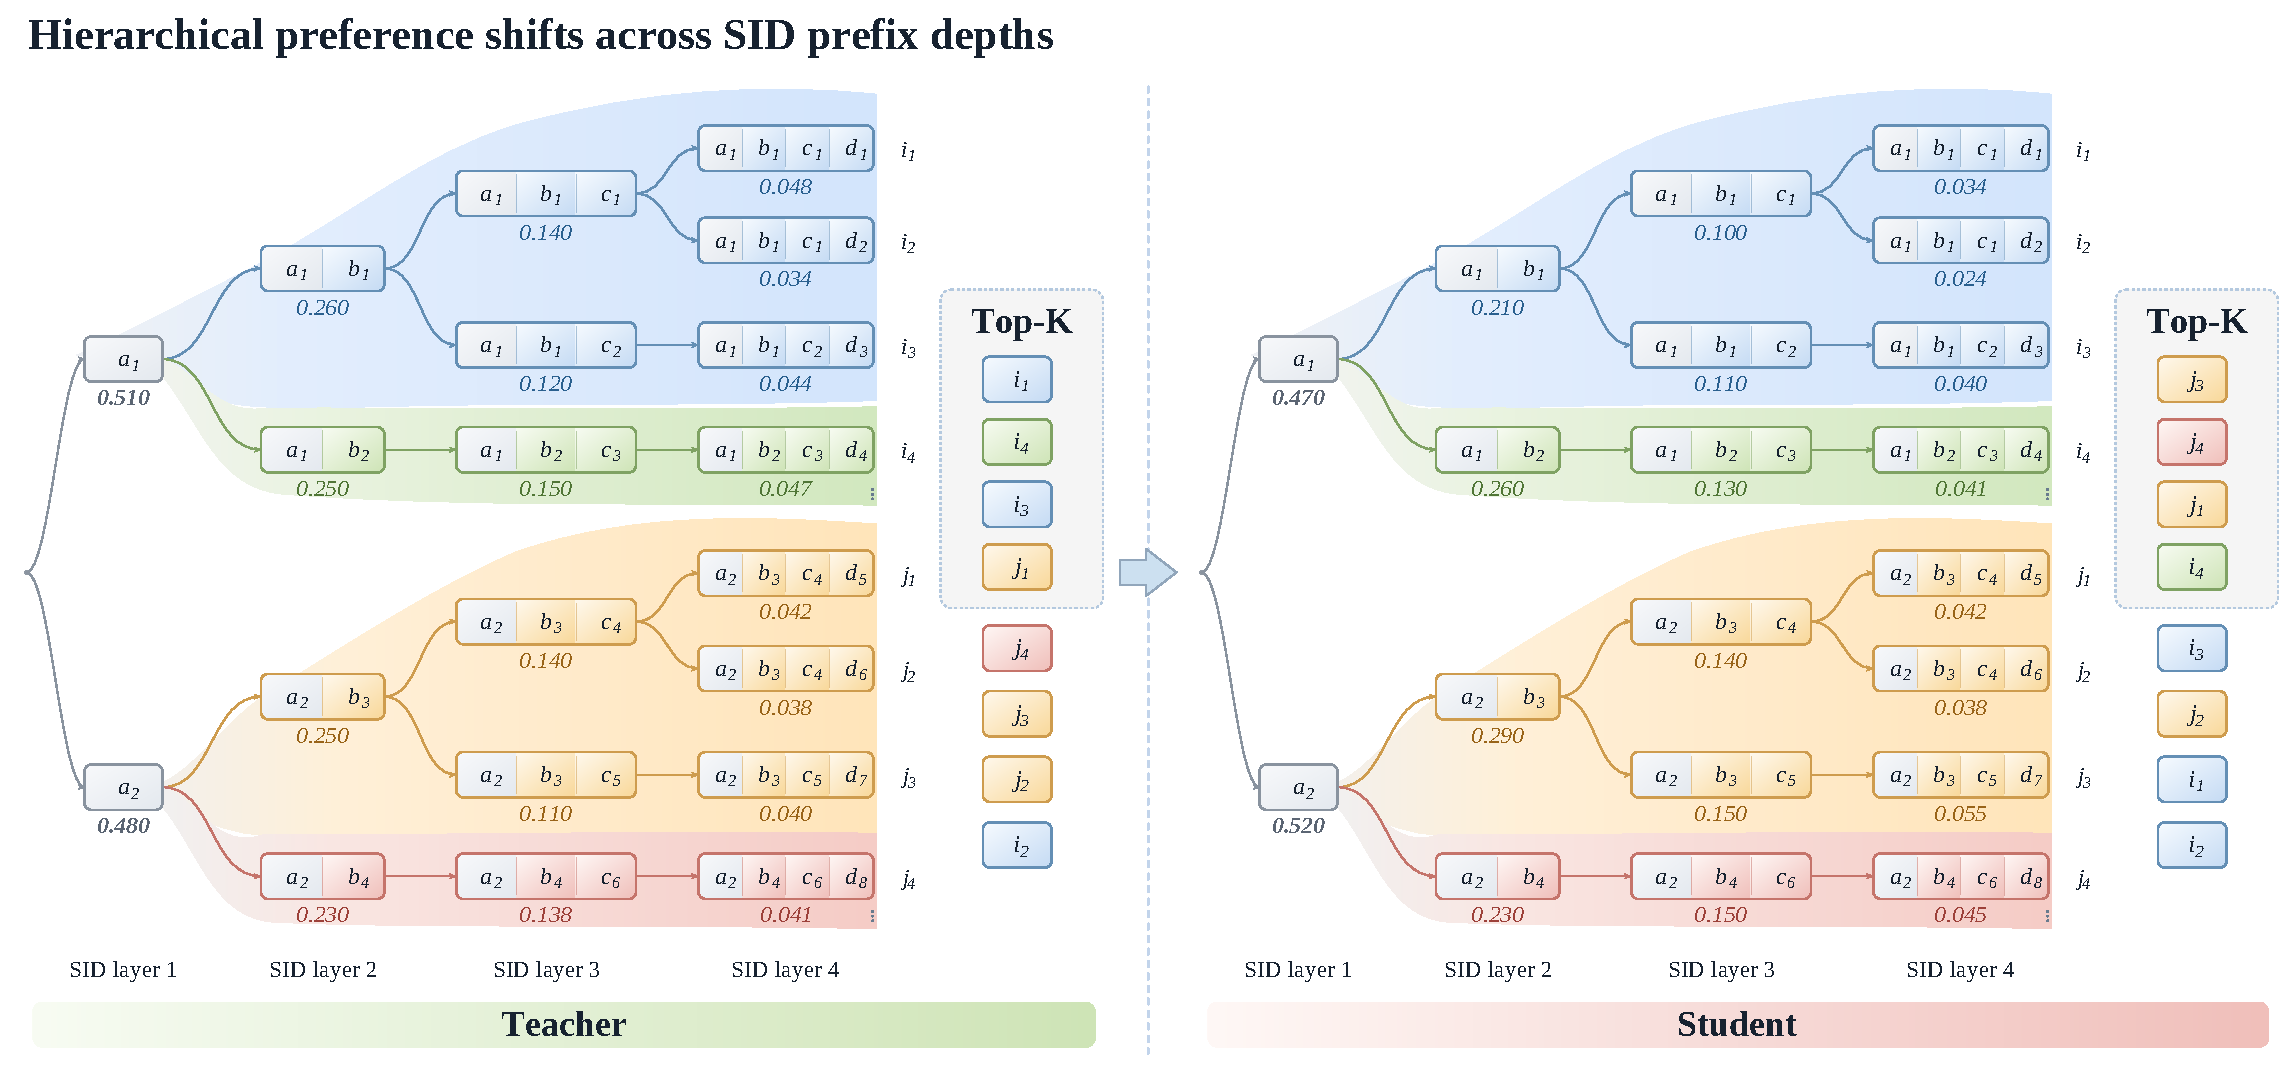
\includegraphics[width=0.64\textwidth]{Figures/diag_hierarchy.pdf}
\caption{Hierarchical candidate-preference mismatch. Teacher and
student assign different preference masses to shared SID prefix
groups. The example is illustrative.}
\Description{Illustration of hierarchical candidate preference mismatch.}
\label{fig:hierarchical}
\end{figure*}


% Figure: H1 statistics (图1.png) -- local vs candidate fit counterexample
% and preferred-prefix disagreement across datasets and students.
\begin{figure*}[t]
\centering
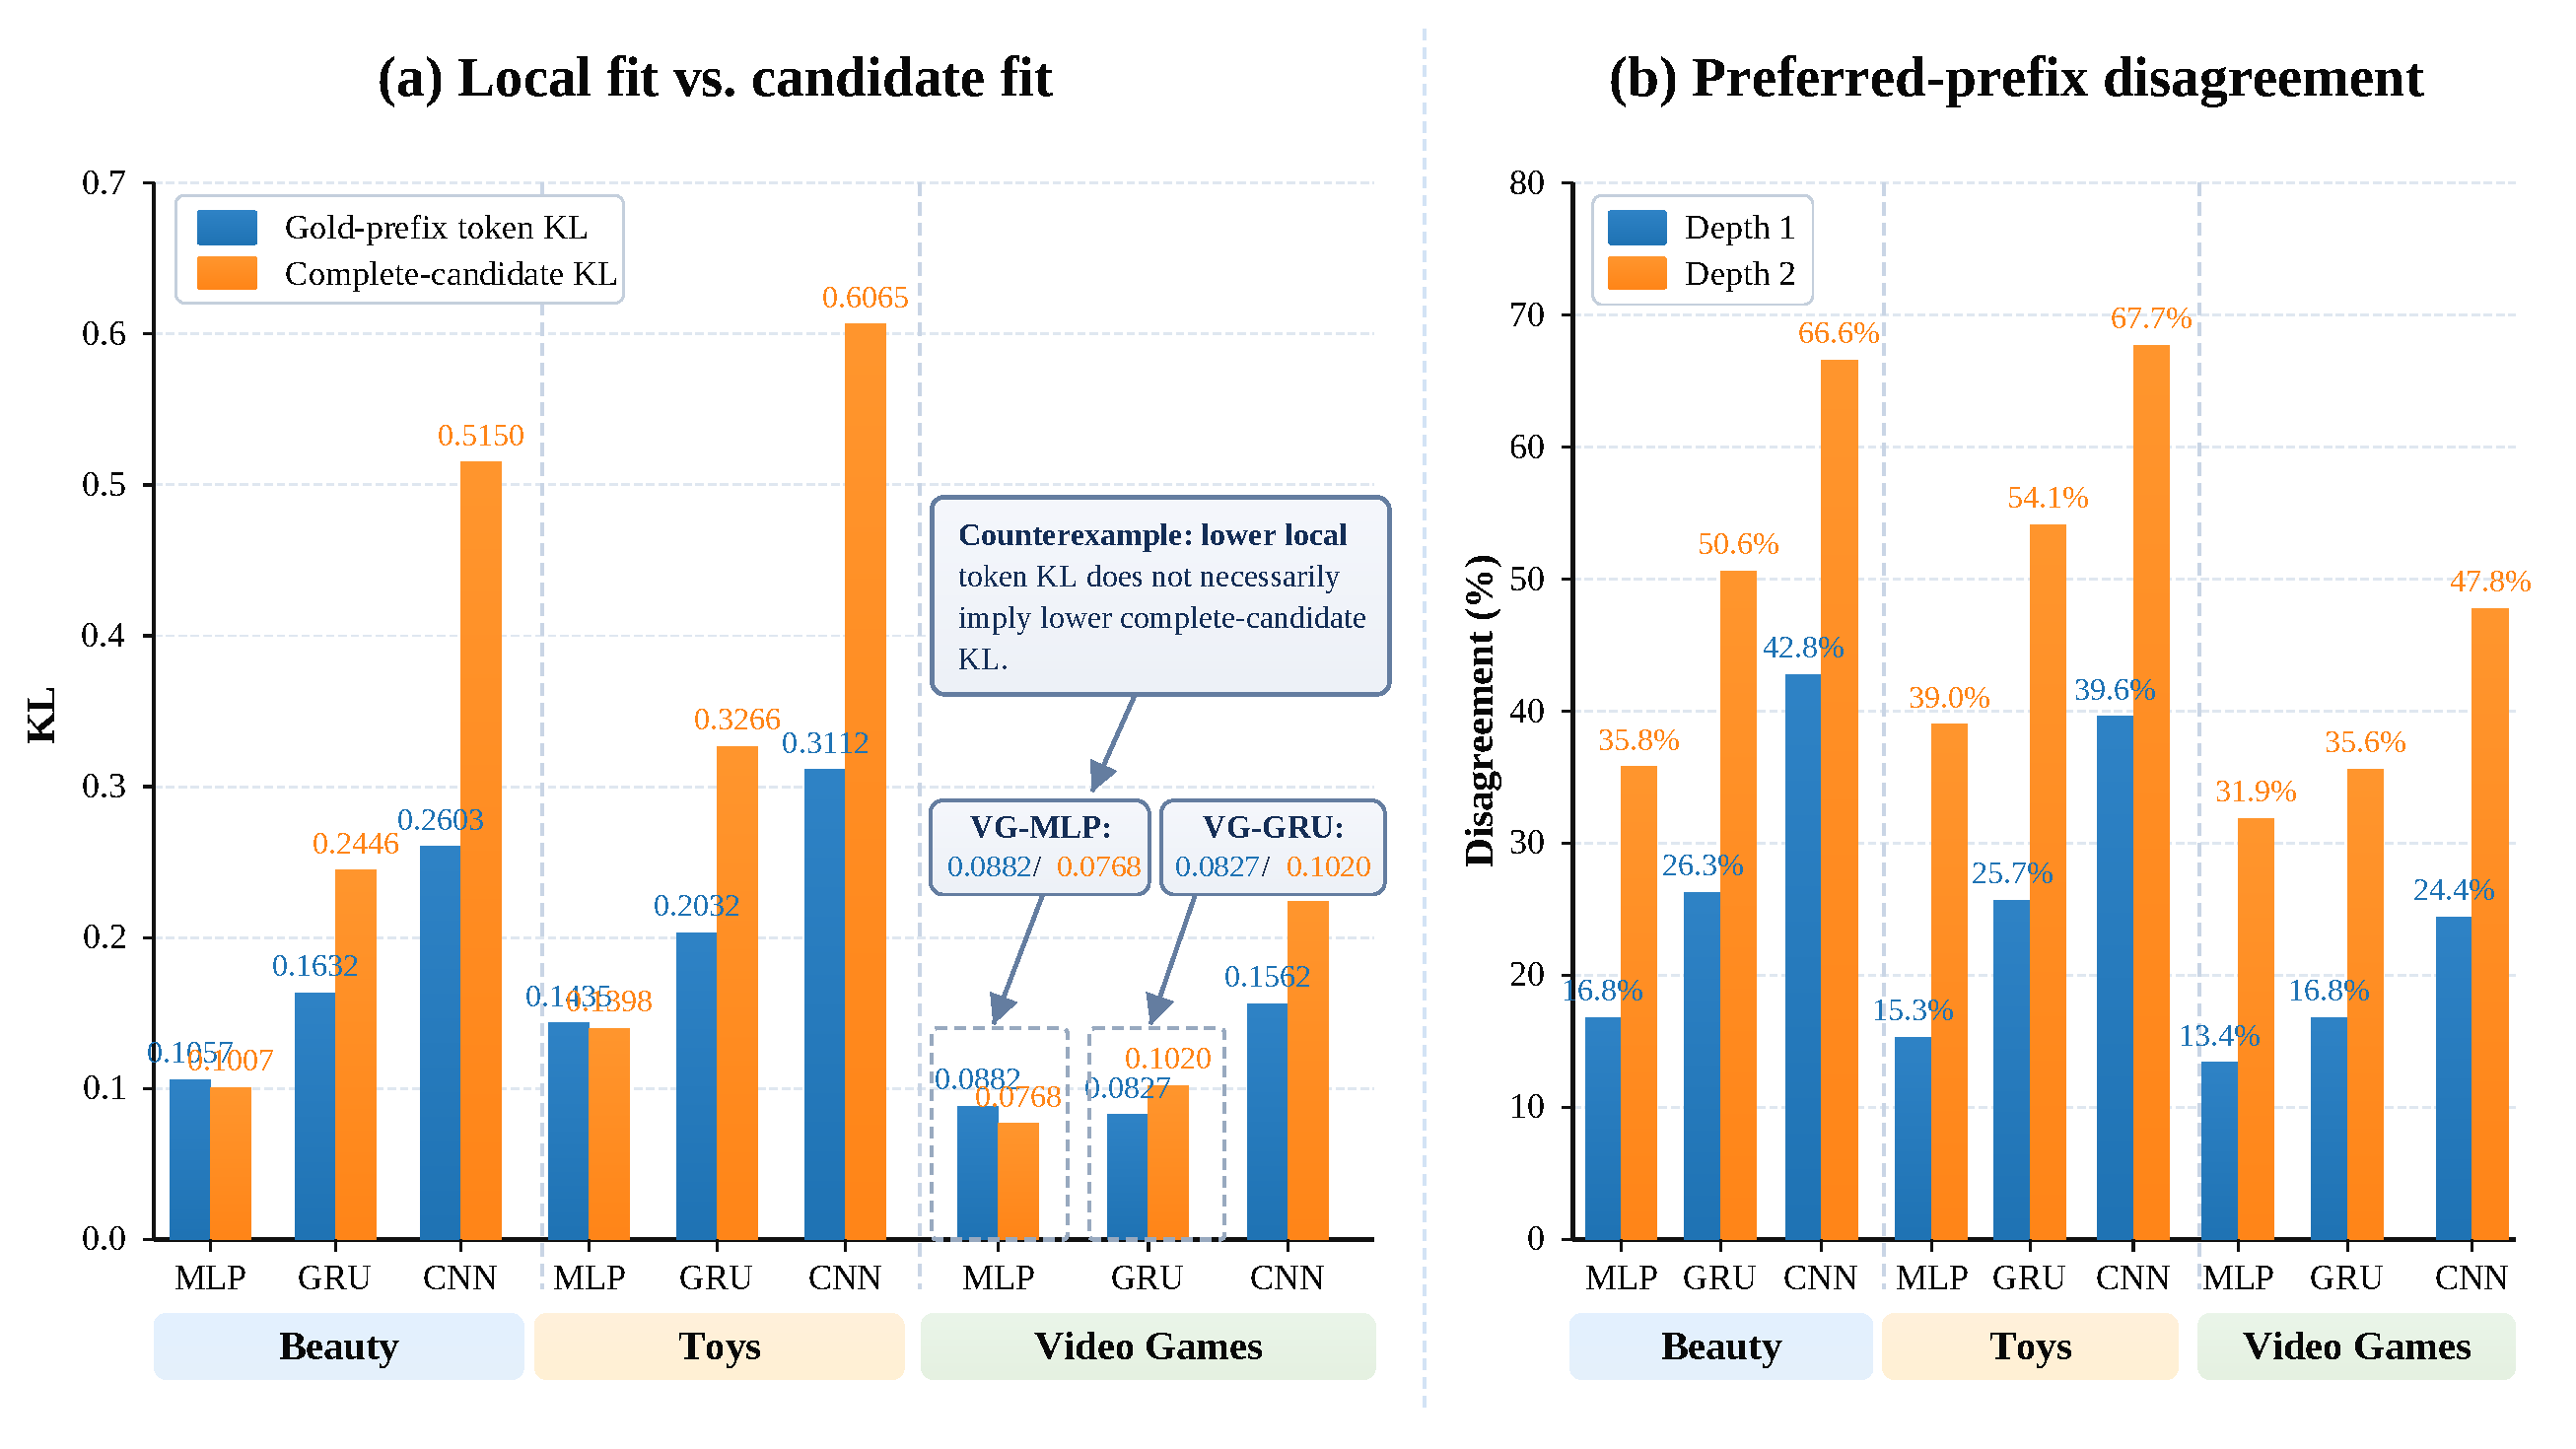
\includegraphics[width=0.62\textwidth]{Figures/fig_stat_h1.pdf}
\caption{Candidate-level and hierarchical preference mismatches.
(a) Local token agreement versus complete-candidate agreement.
(b) Preferred-prefix disagreement across SID depths.}
\Description{Statistics of hierarchical candidate preference mismatch.}
\label{fig:stat-h1}
\end{figure*}


\subsection{Directionally Mixed Cross-Depth Residuals}
\label{sec:diag-d2}

We examine teacher--student relative-score residuals
$r_d=\Delta G_T^{(d)}-\Delta G_S^{(d)}$ on held-out teacher-ordered
candidate pairs. A mixed-sign pair has both a positive and a negative
residual across eligible non-final SID depths; the cancellation ratio
summarizes how signed depth residuals offset one another. Figure~\ref{fig:stat-d12} shows that $75.4\%$--$86.3\%$ of pairs contain both positive and negative depth-wise residuals, while the largest absolute residual is negative in $47.6\%$--$51.3\%$ of cases. Thus, discrepancy magnitude alone does not identify corrections that favor the teacher-preferred ordering. This motivates direction-aware allocation of depth-wise distillation supervision.

Together, hierarchical candidate-preference mismatches and directionally mixed depth residuals motivate the two complementary structural objectives introduced next.

% Figure 3: directional composition of depth-wise relative-score residuals
% (ServeSID_figures_no_pairloss/ServeSID_Figure3_D2_only.png).
\begin{figure*}[t]
\centering
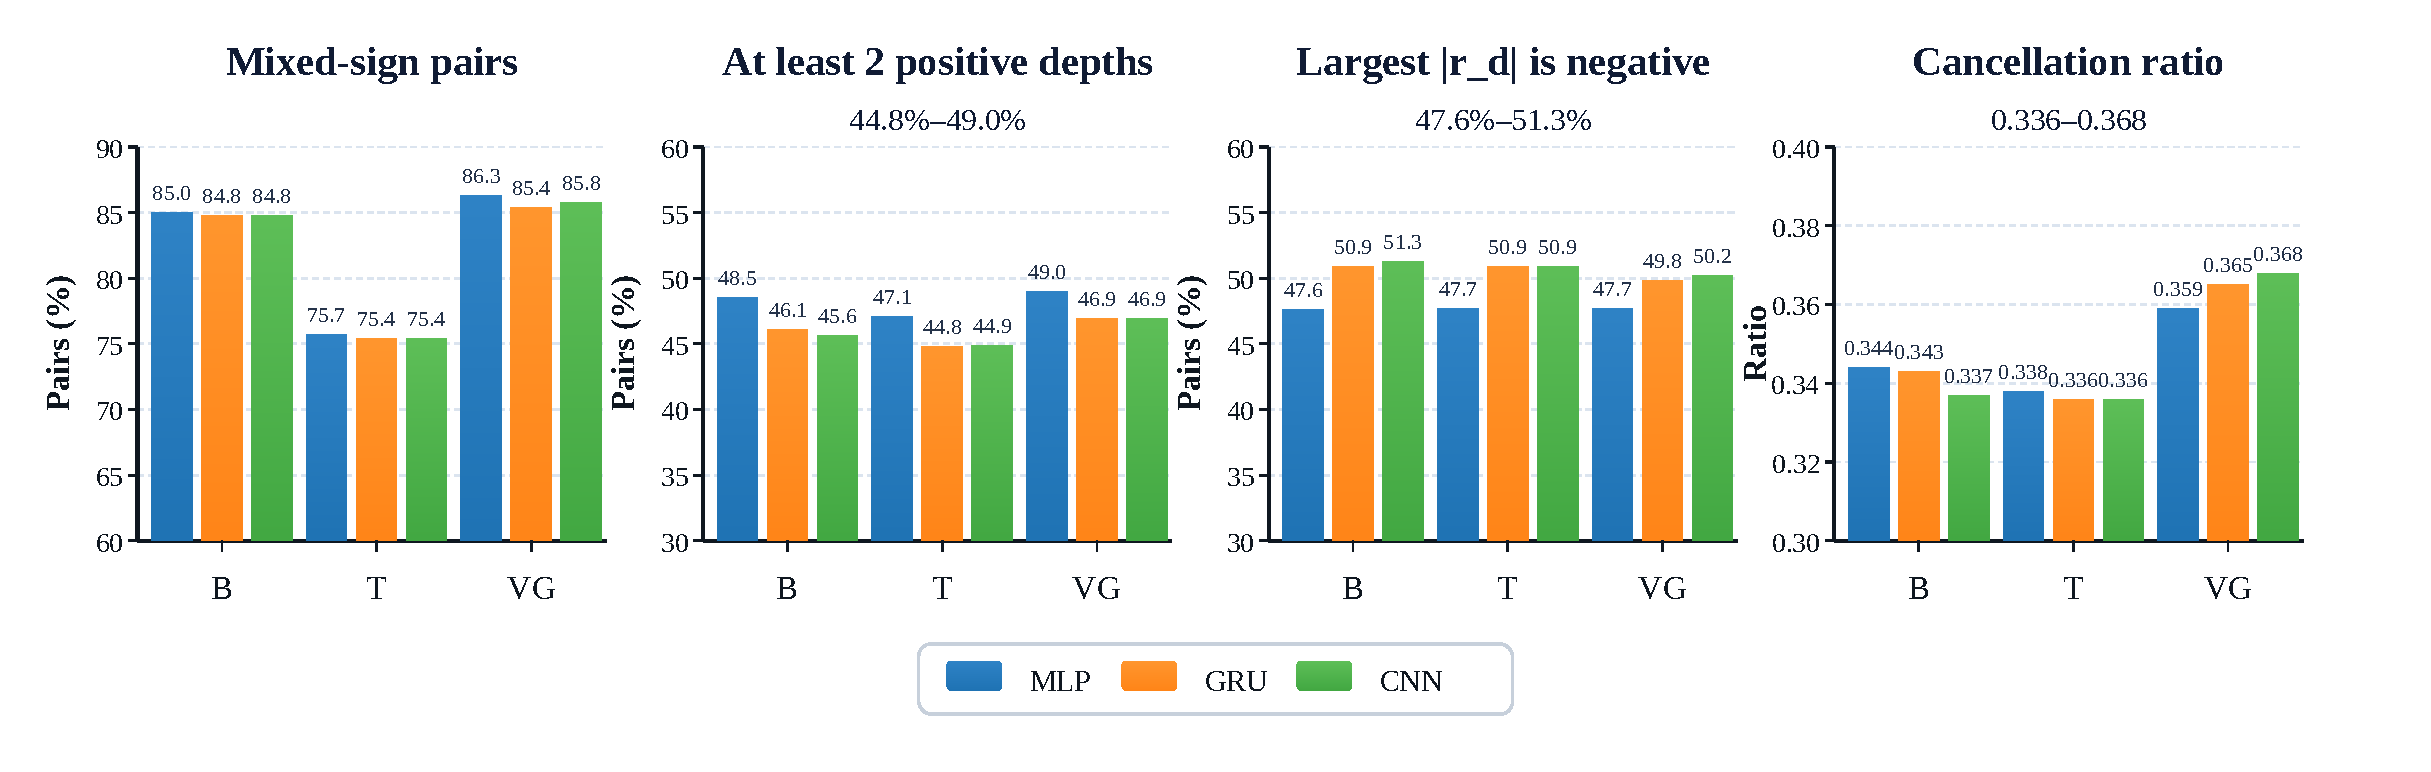
\includegraphics[width=0.85\textwidth]{Figures/fig_stat_d12.pdf}
\caption{Directional composition of depth-wise residuals. Mixed-sign
residuals, positive-residual depths, negative-dominant residuals, and
cancellation ratios across datasets and student architectures.}
\Description{Statistics of the directional composition of depth-wise residuals.}
\label{fig:stat-d12}
\end{figure*}


% Figure 4: directional effects of depth-wise score corrections (image2.svg).
\begin{figure*}[t]
\centering
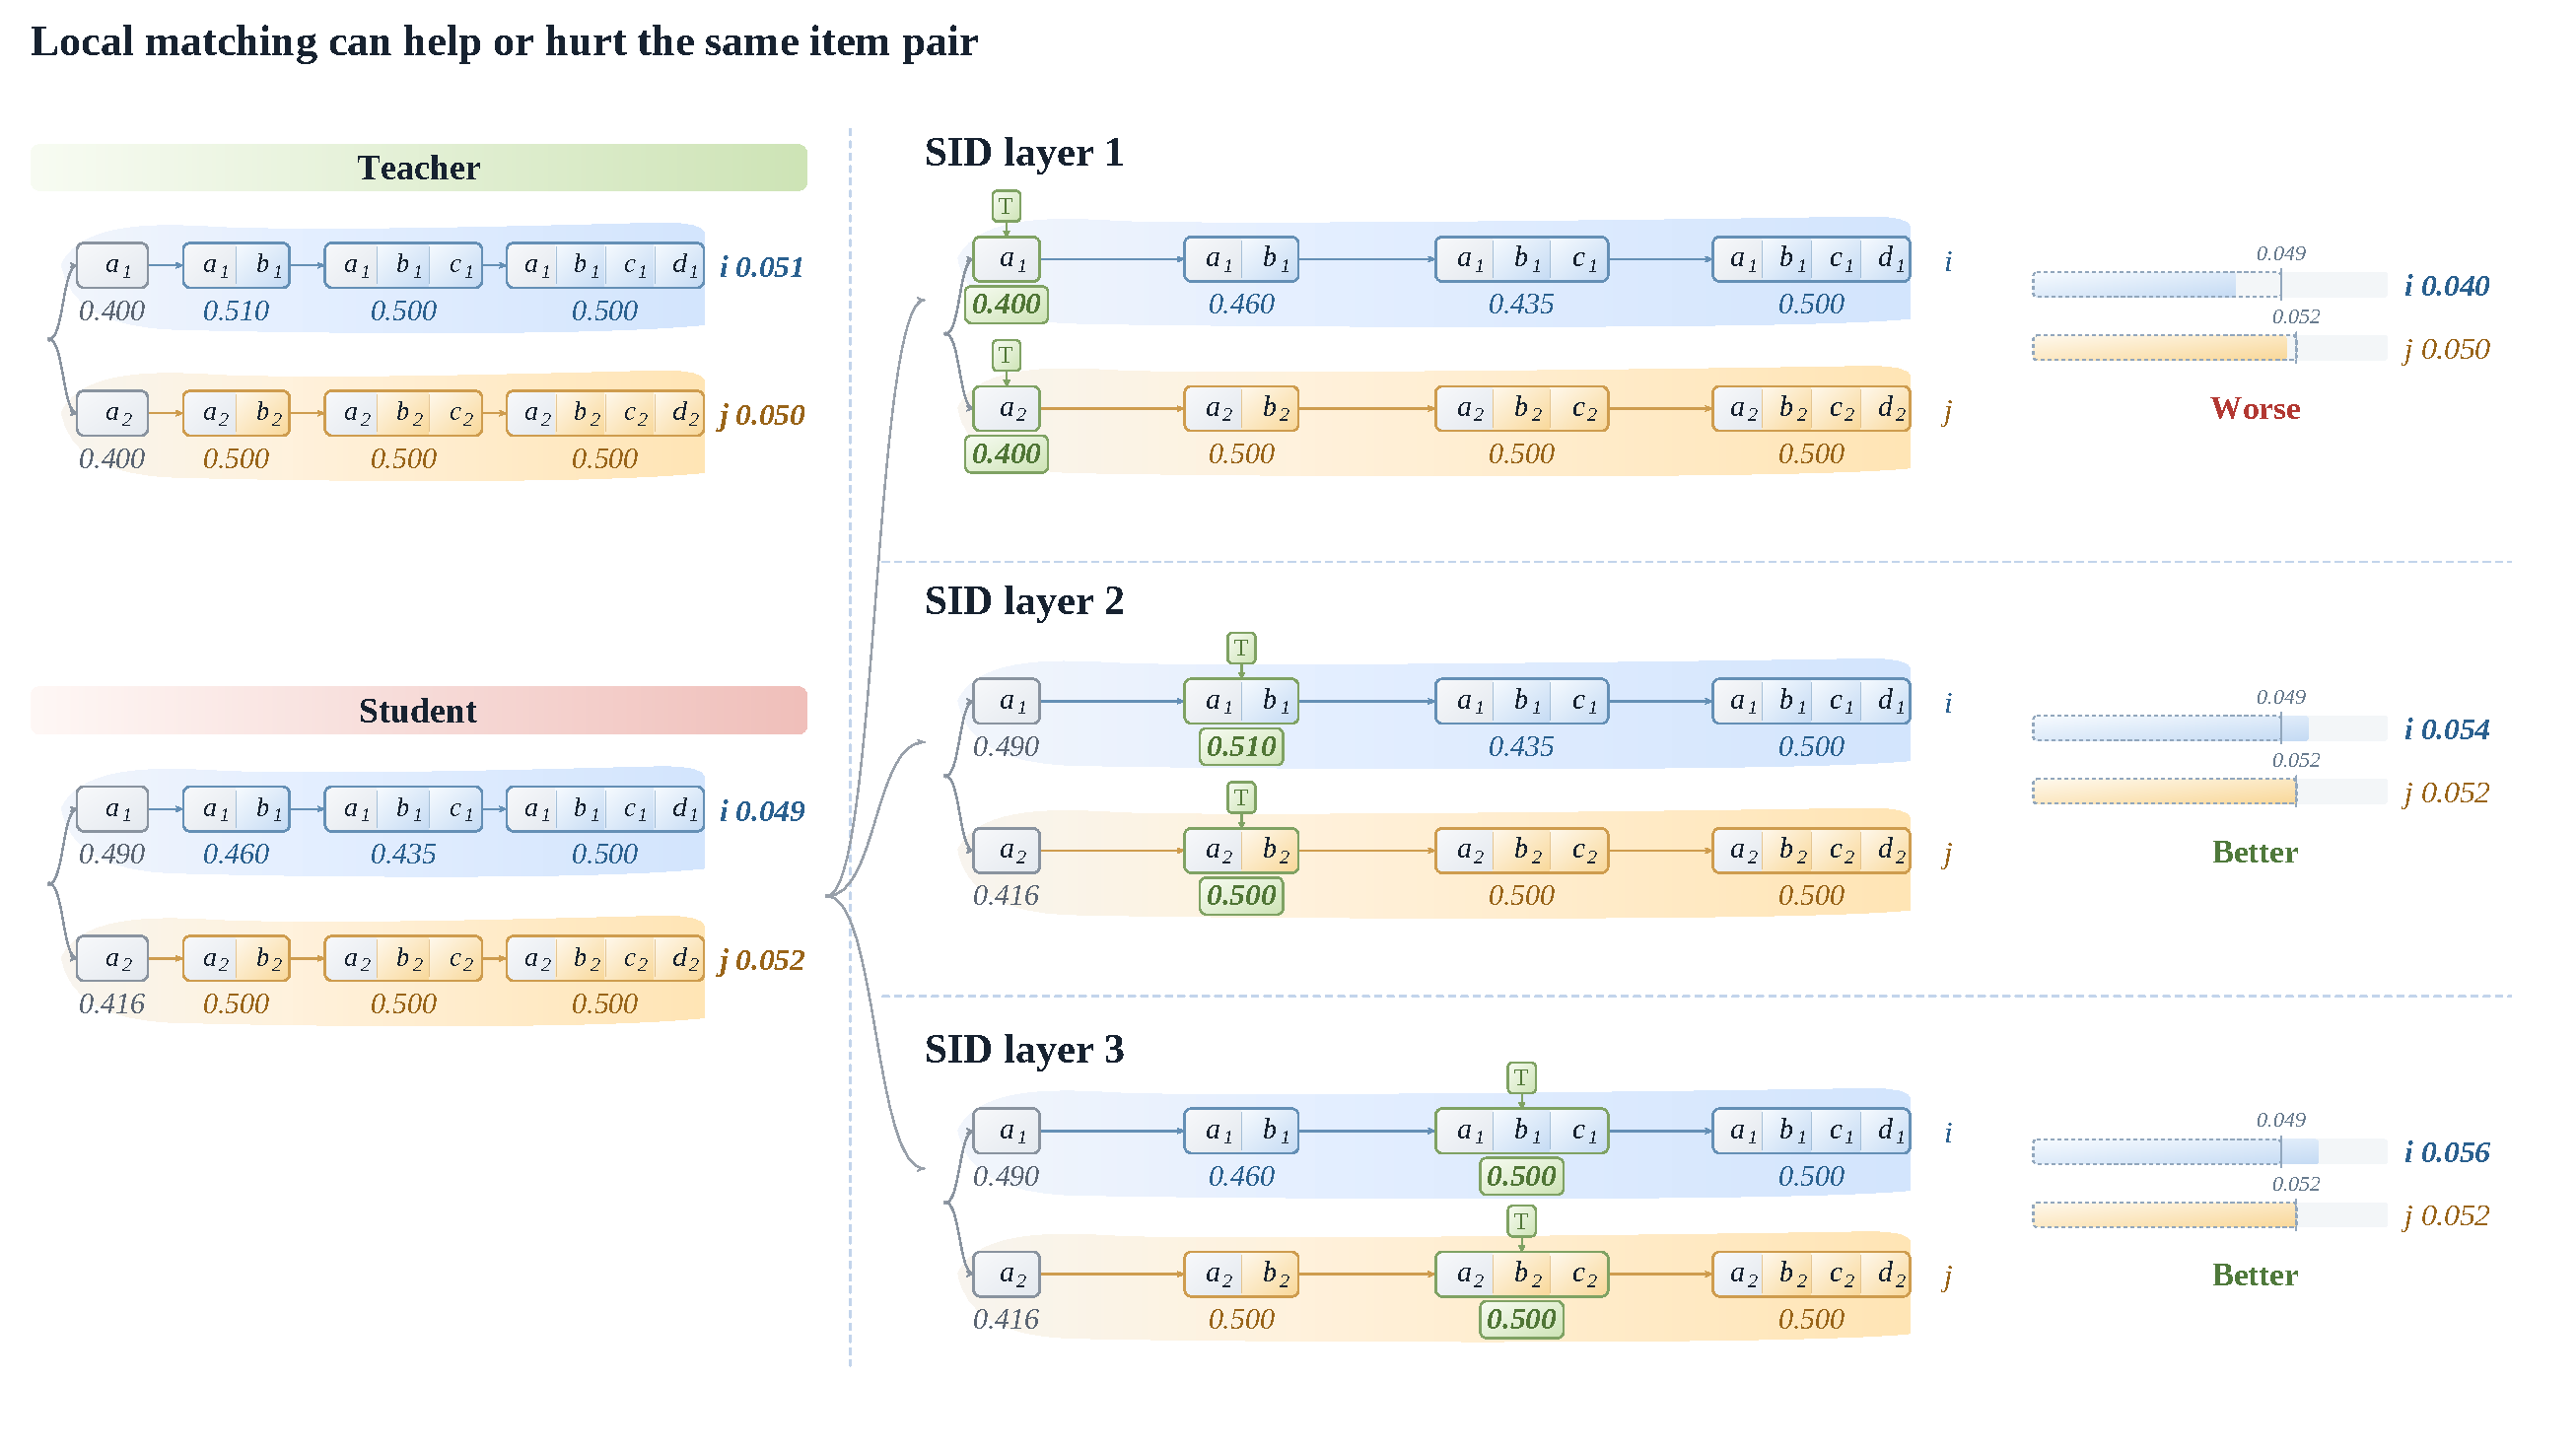
\includegraphics[width=0.90\textwidth]{Figures/diag_replace.pdf}
\caption{Directional effects of depth-wise correction. Replacing a
student increment with its teacher counterpart can increase or
decrease the complete-candidate score gap.}
\Description{Illustration of directional effects of single-depth teacher replacement.}
\label{fig:ranking_depth}
\end{figure*}




\section{\method: Hierarchy-Aligned and Decision-Attributed Distillation}
\label{sec:method}

The frozen teacher proposes complete SID candidates on a common
support. HServe aligns their prefix marginals; DA-CDRS scores
single-depth teacher replacements to allocate relative-score
distillation. Both losses update the same student.

% Editable fallback overview. Replace with Figures/main_method.pdf when final artwork is available.
% Avoid any claims about measured latency/accuracy in this schematic.
\begin{figure*}[t]
\centering
% Reserve the same 53mm plot area for the author's final main_method.pdf.
\begin{minipage}[c][53mm][c]{\textwidth}
\centering
\IfFileExists{Figures/main_method.pdf}{%
  \includegraphics[width=0.98\textwidth,height=53mm,keepaspectratio]{Figures/main_method.pdf}%
}{%
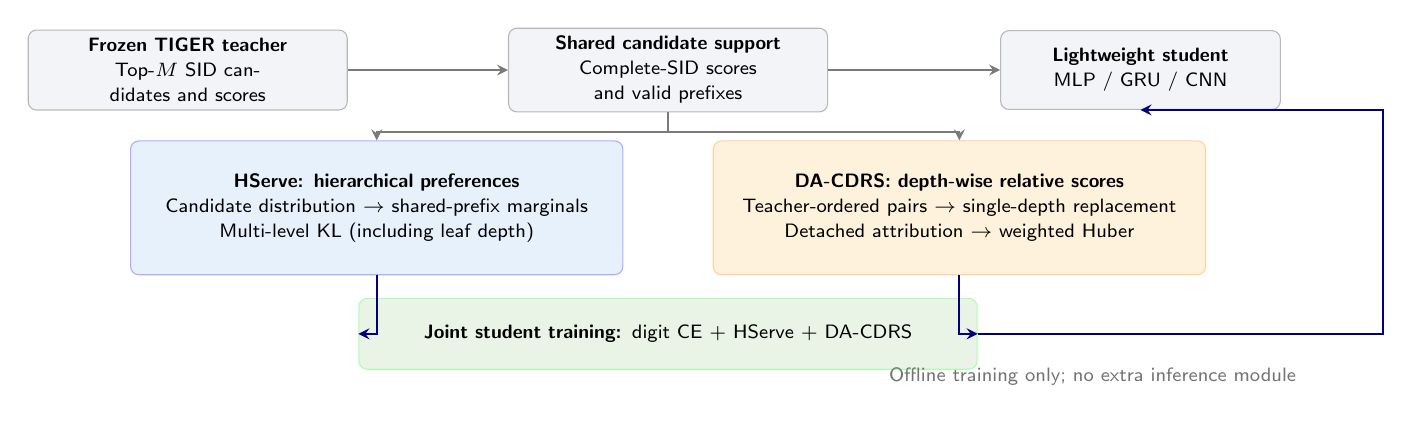
\begin{tikzpicture}[
  >=stealth,
  every node/.style={font=\sffamily\fontsize{7.4}{9}\selectfont},
  frame/.style={draw=black!28,rounded corners=3pt,minimum height=10mm,align=center,inner xsep=5pt,inner ysep=3pt},
  bluebox/.style={frame,fill=catTrad,draw=blue!32},
  orangebox/.style={frame,fill=catGen,draw=orange!35},
  greenbox/.style={frame,fill=catSID,draw=green!32},
  graybox/.style={frame,fill=datasetgray},
  flow/.style={->,draw=black!52,line width=0.75pt},
  training/.style={->,draw=blue!50!black,line width=0.75pt},
]
\node[graybox,text width=37mm] (teacher) at (2.0,0)
  {\textbf{Frozen TIGER teacher}\\Top-$M$ SID candidates and scores};
\node[graybox,text width=37mm] (support) at (8.1,0)
  {\textbf{Shared candidate support}\\Complete-SID scores and valid prefixes};
\node[graybox,text width=32mm] (student) at (14.1,0)
  {\textbf{Lightweight student}\\MLP / GRU / CNN};

\node[bluebox,text width=59mm,minimum height=17mm] (hserve) at (4.4,-1.75)
  {\textbf{HServe: hierarchical preferences}\\Candidate distribution $\rightarrow$ shared-prefix marginals\\Multi-level KL (including leaf depth)};
\node[orangebox,text width=59mm,minimum height=17mm] (da) at (11.8,-1.75)
  {\textbf{DA-CDRS: depth-wise relative scores}\\Teacher-ordered pairs $\rightarrow$ single-depth replacement\\Detached attribution $\rightarrow$ weighted Huber};
\node[greenbox,text width=75mm,minimum height=9mm] (joint) at (8.1,-3.35)
  {\textbf{Joint student training:} digit CE $+$ HServe $+$ DA-CDRS};

\draw[flow] (teacher.east) -- (support.west);
\draw[flow] (support.east) -- (student.west);
\draw[flow] (support.south) -- ++(0,-0.25) -| (hserve.north);
\draw[flow] (support.south) -- ++(0,-0.25) -| (da.north);
\draw[training] (hserve.south) |- (joint.west);
\draw[training] (da.south) |- (joint.east);
\draw[training] (joint.east) -- ++(5.15,0) |- (student.south);
\node[font=\sffamily\fontsize{6.8}{7.8}\selectfont,text=black!55,anchor=east] at (16.2,-3.9)
  {Offline training only; no extra inference module};
\end{tikzpicture}%
}
\end{minipage}
\caption{Overview of \method. HServe aligns complete-candidate and prefix-level preferences; DA-CDRS weights depth-wise relative-score matching using detached single-depth attribution. Both objectives update the same lightweight student offline.}
\Description{Training-only teacher candidate supervision branches into hierarchical candidate-marginal alignment and direction-attributed depth-wise Huber distillation. The jointly trained student retains its original inference architecture.}
\label{fig:method-overview}
\end{figure*}


\subsection{Overall Training Objective}
\label{sec:method-total}

For a training request $u$ with observed next-item SID
$z^{\mathrm{gt}}$, our objective is
\begin{equation}
\mathcal L_{\mathrm{\method}}
=\mathcal L_{\mathrm{digit}}
+\lambda_H\mathcal L_{\mathrm{HServe}}
+\lambda_D\mathcal L_{\mathrm{DA\text{-}CDRS}},
\label{eq:total}
\end{equation}
where $\mathcal L_{\mathrm{digit}}$ is the ground-truth SID
cross-entropy defined in Section~\ref{sec:prelim-base}, and
$\lambda_H,\lambda_D\ge0$ control the structural objectives. Unlike
the baseline, \method\ does not retain a separate gold-prefix
token-KL term. Ground-truth supervision remains necessary because
matching a teacher's preferences does not guarantee relevance to the
observed next item. The following losses operate on teacher-proposed
complete candidates, with gradients applied only to the student.
Request-level objectives are averaged across the training minibatch, and the teacher is fixed throughout optimization, keeping the distillation targets stationary while the student adapts.

\subsection{HServe: Hierarchical Serving-Distribution Alignment}
\label{sec:method-hserve}

\textbf{Shared complete-candidate support.} For each training
request, we obtain the teacher's top-$M$ beam-reachable, valid
complete SIDs and cache the resulting support $\C_M(u)$. Both models
evaluate these same complete sequences using accumulated conditional
log-probabilities $s_m(i\mid u)$, where $m\in\{T,S\}$. Teacher scores can be precomputed, whereas student scores are recomputed as parameters change. We define a distribution normalized within
this support:
\begin{equation}
\pi_{m,M}(i\mid u)=
\frac{\exp(s_m(i\mid u))}
{\sum_{j\in\C_M(u)}\exp(s_m(j\mid u))},
\qquad i\in\C_M(u).
\label{eq:item-dist}
\end{equation}
This normalization makes teacher and student probabilities comparable
over identical candidates. It represents preference
conditional on the selected support rather than over the entire item
catalog, so candidates outside $\C_M(u)$ are not part of this KL
objective; using a common support avoids interpreting differences
caused merely by two models proposing different candidate lists as
distributional mismatch.

\textbf{Hierarchically consistent prefix marginals.} As illustrated
in Figure~\ref{fig:hierarchical}, shared SID prefixes form nested
candidate groups whose preference mass may differ between teacher and
student. A length-$d$ prefix $p$ defines the subset of supported
candidates whose first $d$ codes equal $p$. We aggregate their complete-candidate
probabilities:
\begin{equation}
\pi_{m,M}^{(d)}(p\mid u)=
\sum_{\substack{i\in\C_M(u)\\z_{1:d}^i=p}}
\pi_{m,M}(i\mid u).
\label{eq:prefix-marginal}
\end{equation}
Every candidate contributes to exactly one prefix group at each
depth, so the marginals are normalized and mutually consistent across
depths. At $d=L$, each distinct complete SID corresponds to a leaf
and the marginal reduces to the complete-candidate distribution. At
shallower depths, it captures the total preference mass assigned to
groups of candidates with common initial codes. No auxiliary prefix
predictor is introduced: all marginals are deterministic aggregations
of the same complete-candidate scores. These groupings are defined by
code identity rather than manually assigned product categories.

\textbf{Multi-level alignment.} HServe minimizes the teacher-to-student
KL divergence at every depth:
\begin{equation}
\mathcal L_{\mathrm{HServe}}(u)=
\sum_{d=1}^{L}\alpha_d\,
\KL\!\left(
\pi_{T,M}^{(d)}(\cdot\mid u)\;\|\;
\pi_{S,M}^{(d)}(\cdot\mid u)
\right),\qquad \alpha_d\ge0.
\label{eq:hserve}
\end{equation}
The leaf term ($d=L$) directly aligns complete-item preferences,
addressing the local-to-candidate gap. Shallower terms align probability
mass over shared-prefix groups, addressing hierarchical drift.
Exact leaf-level matching implies agreement at all shallower depths;
these terms provide explicit multi-granularity optimization constraints
rather than independent teacher information. The same student candidate
scores receive gradients from every level, with depth weights
$\alpha_d$ controlling their relative emphasis.

\subsection{DA-CDRS: Decision-Attributed Cross-Depth
Relative-Score Distillation}
\label{sec:method-dacdrs}

\textbf{Cross-cutoff candidate pairs.} We form teacher-ordered pairs
from the fixed candidate list:
\begin{equation}
\mathcal B(u)=\{(i^+,i^-):
\operatorname{rank}_T(i^+\mid u)\le K_{\mathrm{tr}},\;
K_{\mathrm{tr}}<\operatorname{rank}_T(i^-\mid u)\le B\},
\label{eq:pairs}
\end{equation}
where $B\le M$. Pair labels describe teacher preferences, not
ground-truth relevance. For model $m\in\{T,S\}$, the complete score gap is
\begin{equation}
G_m(b)=s_m(i^+\mid u)-s_m(i^-\mid u)
=\sum_{d=1}^{L}\Delta G_m^{(d)}(b),
\label{eq:pairs-gap}
\end{equation}
where
\begin{equation}
\Delta G_m^{(d)}(b)=
\log q_m(z_d^{i^+}\mid u,z_{<d}^{i^+})-
\log q_m(z_d^{i^-}\mid u,z_{<d}^{i^-}),
\label{eq:pairs-inc}
\end{equation}
and $q_T=p_T$ by notation.

\textbf{Decision-attributed depth weighting.} The signed residual is
\begin{equation}
r_d(b)=\Delta G_T^{(d)}(b)-\Delta G_S^{(d)}(b).
\label{eq:residual}
\end{equation}
Shared-prefix increments cancel before the first divergent position
$d_{\mathrm{div}}(b)$. We restrict DA corrections to non-final depths:
\begin{equation}
v_d(b)=\mathbf1[d\ge d_{\mathrm{div}}(b)]
       \mathbf1[d<L].
\label{eq:valid-depth}
\end{equation}
The final SID depth still contributes to the complete score gap but
is not directly corrected by DA-CDRS. As illustrated in
Figure~\ref{fig:ranking_depth}, each hypothetical replacement keeps all
other student increments fixed:
\begin{equation}
\widetilde G_{S,d}(b)=G_S(b)-\Delta G_S^{(d)}(b)
+\Delta G_T^{(d)}(b).
\label{eq:cf-gap}
\end{equation}
We evaluate the complete-pair ordering with
$\ell_{\mathrm{pair}}(G)=\operatorname{softplus}(\mu-G)$,
where $\mu$ is a fixed margin. The positive reduction in this
\emph{evaluation function} defines attribution:
\begin{equation}
A_d(b)=v_d(b)\left[
\ell_{\mathrm{pair}}(G_S(b))-
\ell_{\mathrm{pair}}(\widetilde G_{S,d}(b))
\right]_+.
\label{eq:attribution}
\end{equation}
Detached weights normalize these improvements:
\begin{equation}
w_d(b)=\operatorname{stopgrad}\left(
\frac{A_d(b)}{\sum_{t=1}^{L-1}A_t(b)+\epsilon}
\right).
\label{eq:weights}
\end{equation}
Unlike normalized positive-residual weighting, the magnitude here
depends on the current complete student gap through the nonlinear
pairwise evaluation. Since the function is monotone, positive
attribution still requires $r_d>0$. The replacement is a local score
calculation, not a causal intervention on model parameters. We do not
backpropagate through $\ell_{\mathrm{pair}}$ or directly minimize it.

\textbf{Scale-normalized relative-score correction.} With
depth-specific standard deviations computed from valid \emph{training}
pairs, we set
\begin{equation}
\sigma_d=\max\left(
\operatorname{Std}_{\mathrm{train,valid}}[
\Delta G_T^{(d)}],10^{-4}\right).
\label{eq:scale}
\end{equation}
DA-CDRS optimizes only weighted Huber increment matching:
\begin{equation}
\ell_{\mathrm{DA}}(b)=
\lambda_{\mathrm{corr}}\sum_{d=1}^{L-1}
w_d(b)\,\rho_H\!\left(
\frac{\Delta G_S^{(d)}(b)-\Delta G_T^{(d)}(b)}{\sigma_d}
\right).
\label{eq:correction}
\end{equation}
The request loss averages over $\mathcal B(u)$ and is zero if this
set is empty. If all eligible attributions vanish, that pair adds no
DA correction. The complete-pair Softplus is used \emph{only} to
compute detached weights, never as an independent training loss.
Whether its gap-sensitive allocation improves upon uniform or simple
positive-residual weights requires controlled ablations.

\subsection{Offline Training and Verify-Free Inference}
\label{sec:method-train-inf}

We construct teacher proposal lists, candidate scores, pair relations,
and teacher increment statistics from training requests only. The frozen teacher's data are cached; student scores, marginals, replacements, and attribution weights are computed during optimization. No validation or test request contributes teacher targets to the training loss.

At deployment, all teacher-dependent caches and distillation
computations are discarded. The student retains one history-encoding
pass, depth-wise SID prediction, validity masking, and constrained
beam expansion. Consequently, the deployed student retains the original verify-free inference graph without introducing teacher-dependent scoring, auxiliary prediction heads, or reranking stages. The proposed objectives modify only the offline training procedure and do not constitute a new decoding algorithm. Offline cache
generation, storage, and additional student scoring nevertheless
increase training-side cost; they should be reported separately from
serving latency. The method targets recommendation quality under an
unchanged verify-free inference graph, not a guaranteed preservation
of every teacher Top-$K$ item.

\section{Experiments}
\label{sec:exp}

% Place wide experiment tables early so they float before References.
% AUTO-GENERATED by scripts/gen_tables.py -- do not edit by hand.
\begin{table*}[t]
\centering
\begingroup
\fontsize{7.0}{8.6}\selectfont
\setlength{\tabcolsep}{1.1pt}
\renewcommand{\arraystretch}{1.22}
\noindent\makebox[\textwidth][s]{\fontsize{12}{13}\selectfont\bfseries Recommendation Performance\hfill\fontsize{7}{8}\selectfont\normalfont\color{gray}Recall / NDCG at $K \in \{5,10\}$}\par
\vspace{2pt}
\noindent\rule{\textwidth}{0.5pt}\par\vspace{-6pt}
\begin{tabular*}{\textwidth}{@{\extracolsep{\fill}} l l l *{12}{c} @{} }
\toprule
\textbf{Dataset} & \textbf{Category} & \textbf{Method} & \multicolumn{4}{c}{\textbf{MLP}} & \multicolumn{4}{c}{\textbf{GRU}} & \multicolumn{4}{c}{\textbf{CNN}} \\
\cmidrule(lr){4-7}\cmidrule(lr){8-11}\cmidrule(l){12-15}
 & & & R@5 & N@5 & R@10 & N@10 & R@5 & N@5 & R@10 & N@10 & R@5 & N@5 & R@10 & N@10 \\
\midrule
\rowcolor{rowAlt}\cellcolor{white} & \cellcolor{white} & RD & 0.0422 & 0.0281 & 0.0657 & 0.0357 & \second{0.0433} & 0.0285 & \second{0.0671} & \second{0.0362} & 0.0419 & 0.0274 & 0.0649 & 0.0348 \\
\cellcolor{white} & \cellcolor{white} & RRD & 0.0430 & \second{0.0287} & 0.0659 & 0.0361 & 0.0422 & 0.0281 & 0.0664 & 0.0359 & \second{0.0420} & \second{0.0281} & 0.0649 & \second{0.0354} \\
\rowcolor{rowAlt}\cellcolor{white} & \cellcolor{white}\multirow{-3}{*}{\catrect{catTrad}{29pt}{Traditional\\Recommendation KD}} & RCE-KD & \second{0.0434} & 0.0286 & 0.0666 & \second{0.0363} & 0.0432 & \second{0.0286} & \second{0.0671} & 0.0361 & 0.0409 & 0.0276 & \second{0.0651} & \second{0.0354} \\
\addlinespace[1.6pt]
\cellcolor{white} & \cellcolor{white} & GKD & 0.0428 & 0.0286 & \second{0.0668} & \second{0.0363} & 0.0416 & 0.0281 & 0.0656 & 0.0358 & 0.0380 & 0.0254 & 0.0580 & 0.0319 \\
\rowcolor{rowAlt}\cellcolor{white} & \cellcolor{white}\multirow{-2}{*}{\catrect{catGen}{19pt}{General autoregressive\\/ LLM KD}} & DistiLLM-2 & 0.0428 & \second{0.0287} & 0.0666 & 0.0361 & 0.0416 & 0.0281 & 0.0656 & 0.0358 & 0.0380 & 0.0254 & 0.0580 & 0.0319 \\
\addlinespace[1.6pt]
\cellcolor{white} & \cellcolor{white} & SID-MLP (base KD) & 0.0429 & 0.0282 & 0.0660 & 0.0356 & 0.0416 & 0.0281 & 0.0656 & 0.0358 & 0.0380 & 0.0254 & 0.0580 & 0.0319 \\
\rowcolor{rowAlt}\cellcolor{white} & \cellcolor{white} & SmartGR & \second{0.0434} & 0.0286 & \second{0.0668} & \second{0.0363} & 0.0426 & \second{0.0286} & 0.0669 & 0.0361 & 0.0374 & 0.0250 & 0.0594 & 0.0320 \\
\rowcolor{serveRow}\cellcolor{white}\multirow{-8}{*}{\textbf{\fontsize{9}{10}\selectfont Beauty}} & \cellcolor{white}\multirow{-3}{*}{\catrect{catSID}{29pt}{SID-based generative\\recommendation KD}} & \textbf{ServeSID} & \textbf{0.0442} & \textbf{0.0292} & \textbf{0.0679} & \textbf{0.0369} & \textbf{0.0441} & \textbf{0.0291} & \textbf{0.0682} & \textbf{0.0368} & \textbf{0.0437} & \textbf{0.0288} & \textbf{0.0686} & \textbf{0.0368} \\
\midrule
\rowcolor{rowAlt}\cellcolor{white} & \cellcolor{white} & RD & 0.0380 & 0.0234 & 0.0615 & 0.0309 & 0.0381 & 0.0245 & 0.0614 & 0.0318 & \second{0.0380} & \second{0.0241} & \second{0.0603} & \second{0.0312} \\
\cellcolor{white} & \cellcolor{white} & RRD & \second{0.0396} & \second{0.0245} & 0.0625 & 0.0319 & 0.0381 & 0.0245 & \second{0.0622} & 0.0322 & 0.0378 & 0.0239 & 0.0585 & 0.0306 \\
\rowcolor{rowAlt}\cellcolor{white} & \cellcolor{white}\multirow{-3}{*}{\catrect{catTrad}{29pt}{Traditional\\Recommendation KD}} & RCE-KD & 0.0387 & 0.0244 & \second{0.0631} & \second{0.0324} & 0.0380 & \second{0.0246} & \second{0.0622} & \second{0.0324} & 0.0364 & 0.0232 & 0.0587 & 0.0303 \\
\addlinespace[1.6pt]
\cellcolor{white} & \cellcolor{white} & GKD & 0.0373 & 0.0237 & 0.0627 & 0.0318 & \second{0.0382} & 0.0243 & 0.0613 & 0.0316 & 0.0328 & 0.0210 & 0.0533 & 0.0276 \\
\rowcolor{rowAlt}\cellcolor{white} & \cellcolor{white}\multirow{-2}{*}{\catrect{catGen}{19pt}{General autoregressive\\/ LLM KD}} & DistiLLM-2 & 0.0375 & 0.0238 & 0.0614 & 0.0315 & 0.0367 & 0.0233 & 0.0565 & 0.0296 & 0.0328 & 0.0210 & 0.0533 & 0.0276 \\
\addlinespace[1.6pt]
\cellcolor{white} & \cellcolor{white} & SID-MLP (base KD) & 0.0374 & 0.0235 & 0.0626 & 0.0315 & 0.0367 & 0.0233 & 0.0565 & 0.0296 & 0.0328 & 0.0210 & 0.0533 & 0.0276 \\
\rowcolor{rowAlt}\cellcolor{white} & \cellcolor{white} & SmartGR & 0.0381 & 0.0241 & 0.0623 & 0.0319 & \second{0.0382} & 0.0242 & 0.0604 & 0.0314 & 0.0329 & 0.0206 & 0.0520 & 0.0267 \\
\rowcolor{serveRow}\cellcolor{white}\multirow{-8}{*}{\textbf{\fontsize{9}{10}\selectfont Toys}} & \cellcolor{white}\multirow{-3}{*}{\catrect{catSID}{29pt}{SID-based generative\\recommendation KD}} & \textbf{ServeSID} & \textbf{0.0408} & \textbf{0.0254} & \textbf{0.0644} & \textbf{0.0330} & \textbf{0.0388} & \textbf{0.0250} & \textbf{0.0650} & \textbf{0.0334} & \textbf{0.0398} & \textbf{0.0250} & \textbf{0.0639} & \textbf{0.0328} \\
\midrule
\rowcolor{rowAlt}\cellcolor{white} & \cellcolor{white} & RD & 0.0575 & 0.0372 & 0.0927 & 0.0485 & 0.0595 & 0.0388 & 0.0938 & 0.0498 & 0.0580 & 0.0373 & \second{0.0921} & 0.0483 \\
\cellcolor{white} & \cellcolor{white} & RRD & 0.0592 & \second{0.0390} & 0.0918 & 0.0496 & 0.0596 & 0.0393 & 0.0892 & 0.0490 & \second{0.0591} & \second{0.0389} & 0.0884 & 0.0483 \\
\rowcolor{rowAlt}\cellcolor{white} & \cellcolor{white}\multirow{-3}{*}{\catrect{catTrad}{29pt}{Traditional\\Recommendation KD}} & RCE-KD & 0.0593 & 0.0388 & 0.0926 & \second{0.0497} & 0.0595 & \second{0.0394} & 0.0938 & \second{0.0503} & 0.0589 & 0.0387 & 0.0919 & \second{0.0493} \\
\addlinespace[1.6pt]
\cellcolor{white} & \cellcolor{white} & GKD & 0.0593 & 0.0388 & \second{0.0929} & 0.0496 & \second{0.0597} & 0.0393 & 0.0937 & 0.0502 & 0.0569 & 0.0370 & 0.0896 & 0.0475 \\
\rowcolor{rowAlt}\cellcolor{white} & \cellcolor{white}\multirow{-2}{*}{\catrect{catGen}{19pt}{General autoregressive\\/ LLM KD}} & DistiLLM-2 & \second{0.0594} & 0.0387 & 0.0927 & 0.0494 & 0.0596 & 0.0392 & \second{0.0939} & \second{0.0503} & 0.0587 & 0.0384 & 0.0914 & 0.0489 \\
\addlinespace[1.6pt]
\cellcolor{white} & \cellcolor{white} & SID-MLP (base KD) & 0.0588 & 0.0383 & 0.0922 & 0.0488 & 0.0591 & 0.0389 & 0.0935 & 0.0499 & 0.0553 & 0.0358 & 0.0870 & 0.0460 \\
\rowcolor{rowAlt}\cellcolor{white} & \cellcolor{white} & SmartGR & 0.0593 & 0.0388 & \second{0.0929} & 0.0496 & 0.0594 & 0.0391 & 0.0933 & 0.0500 & 0.0549 & 0.0359 & 0.0870 & 0.0462 \\
\rowcolor{serveRow}\cellcolor{white}\multirow{-8}{*}{\textbf{\fontsize{9}{10}\selectfont VG}} & \cellcolor{white}\multirow{-3}{*}{\catrect{catSID}{29pt}{SID-based generative\\recommendation KD}} & \textbf{ServeSID} & \textbf{0.0604} & \textbf{0.0396} & \textbf{0.0944} & \textbf{0.0505} & \textbf{0.0607} & \textbf{0.0400} & \textbf{0.0954} & \textbf{0.0512} & \textbf{0.0605} & \textbf{0.0399} & \textbf{0.0944} & \textbf{0.0508} \\
\bottomrule
\end{tabular*}
\endgroup
\par\vspace{3pt}{\color{gray}\fontsize{6.3}{7.5}\selectfont Coral: global best; gray: global second (per dataset $\times$ student $\times$ metric; ties included).}\par
\caption{Overall Top-$K$ recommendation performance across three datasets and three student architectures. Methods are grouped by family.}
\label{tab:main-all}
\end{table*}

% AUTO-GENERATED by scripts/gen_tables.py -- do not edit by hand.
\begin{table*}[t]
\centering
\caption{Ablation of HServe and DA-CDRS across three datasets and student architectures. Colored arm labels distinguish configurations; coral highlights the full model. Bold and gray indicate best and second-best results (ties included).}
\label{tab:ablation}
\begingroup
\fontsize{7.0}{8.6}\selectfont
\setlength{\tabcolsep}{1.1pt}
\renewcommand{\arraystretch}{1.12}
\begin{tabular*}{\textwidth}{@{\extracolsep{\fill}} l l *{12}{c} @{} }
\toprule
\textbf{Dataset} & \textbf{Arm} & \multicolumn{4}{c}{\textbf{MLP}} & \multicolumn{4}{c}{\textbf{GRU}} & \multicolumn{4}{c}{\textbf{CNN}} \\
\cmidrule(lr){3-6}\cmidrule(lr){7-10}\cmidrule(l){11-14}
 & & R@5 & N@5 & R@10 & N@10 & R@5 & N@5 & R@10 & N@10 & R@5 & N@5 & R@10 & N@10 \\
\midrule
\rowcolor{rowAlt}\cellcolor{white} & \ablatag{datasetgray}{SID-MLP (base KD)} & 0.0429 & 0.0282 & 0.0660 & 0.0356 & 0.0416 & 0.0281 & 0.0656 & 0.0358 & 0.0380 & 0.0254 & 0.0580 & 0.0319 \\
\cellcolor{white} & \ablatag{catTrad}{d4-only KL} & 0.0431 & 0.0283 & 0.0663 & 0.0359 & 0.0422 & 0.0283 & 0.0660 & 0.0360 & 0.0402 & 0.0266 & 0.0625 & 0.0348 \\
\rowcolor{rowAlt}\cellcolor{white} & \ablatag{catGen}{DA-CDRS only} & 0.0435 & 0.0286 & 0.0672 & 0.0362 & 0.0430 & 0.0286 & 0.0673 & 0.0364 & 0.0414 & 0.0273 & 0.0652 & 0.0359 \\
\cellcolor{white} & \ablatag{catTrad}{HServe only} & 0.0436 & \second{0.0287} & 0.0670 & 0.0363 & 0.0431 & 0.0286 & 0.0671 & 0.0364 & 0.0418 & 0.0276 & 0.0656 & 0.0360 \\
\rowcolor{rowAlt}\cellcolor{white} & \ablatag{catSID}{HServe + Uniform} & \second{0.0437} & 0.0286 & \second{0.0673} & \second{0.0364} & \second{0.0437} & \second{0.0287} & \second{0.0674} & \second{0.0365} & \second{0.0423} & \second{0.0280} & \second{0.0669} & \second{0.0362} \\
\rowcolor{serveRow}\cellcolor{white}\multirow{-6}{*}{\textbf{\fontsize{9}{10}\selectfont Beauty}} & \textbf{\method (full)} & \textbf{0.0442} & \textbf{0.0292} & \textbf{0.0679} & \textbf{0.0369} & \textbf{0.0441} & \textbf{0.0291} & \textbf{0.0682} & \textbf{0.0368} & \textbf{0.0437} & \textbf{0.0288} & \textbf{0.0686} & \textbf{0.0368} \\
\midrule
\rowcolor{rowAlt}\cellcolor{white} & \ablatag{datasetgray}{SID-MLP (base KD)} & 0.0374 & 0.0235 & 0.0626 & 0.0315 & 0.0367 & 0.0233 & 0.0565 & 0.0296 & 0.0328 & 0.0210 & 0.0533 & 0.0276 \\
\cellcolor{white} & \ablatag{catTrad}{d4-only KL} & 0.0379 & 0.0237 & 0.0628 & 0.0317 & 0.0369 & 0.0237 & 0.0594 & 0.0313 & 0.0354 & 0.0225 & 0.0566 & 0.0305 \\
\rowcolor{rowAlt}\cellcolor{white} & \ablatag{catGen}{DA-CDRS only} & 0.0389 & 0.0246 & 0.0638 & 0.0324 & 0.0377 & 0.0241 & 0.0622 & 0.0323 & 0.0370 & 0.0236 & 0.0598 & 0.0322 \\
\cellcolor{white} & \ablatag{catTrad}{HServe only} & 0.0390 & 0.0245 & 0.0633 & 0.0323 & 0.0379 & 0.0243 & 0.0630 & 0.0325 & 0.0375 & 0.0238 & 0.0606 & 0.0320 \\
\rowcolor{rowAlt}\cellcolor{white} & \ablatag{catSID}{HServe + Uniform} & \second{0.0395} & \second{0.0248} & \second{0.0640} & \second{0.0325} & \second{0.0381} & \second{0.0247} & \second{0.0642} & \second{0.0328} & \second{0.0382} & \second{0.0242} & \second{0.0630} & \second{0.0323} \\
\rowcolor{serveRow}\cellcolor{white}\multirow{-6}{*}{\textbf{\fontsize{9}{10}\selectfont Toys}} & \textbf{\method (full)} & \textbf{0.0408} & \textbf{0.0254} & \textbf{0.0644} & \textbf{0.0330} & \textbf{0.0388} & \textbf{0.0250} & \textbf{0.0650} & \textbf{0.0334} & \textbf{0.0398} & \textbf{0.0250} & \textbf{0.0639} & \textbf{0.0328} \\
\midrule
\rowcolor{rowAlt}\cellcolor{white} & \ablatag{datasetgray}{SID-MLP (base KD)} & 0.0588 & 0.0383 & 0.0922 & 0.0488 & 0.0591 & 0.0389 & 0.0935 & 0.0499 & 0.0553 & 0.0358 & 0.0870 & 0.0460 \\
\cellcolor{white} & \ablatag{catTrad}{d4-only KL} & 0.0589 & 0.0384 & 0.0925 & 0.0491 & 0.0593 & 0.0390 & 0.0937 & 0.0502 & 0.0570 & 0.0370 & 0.0888 & 0.0488 \\
\rowcolor{rowAlt}\cellcolor{white} & \ablatag{catGen}{DA-CDRS only} & 0.0595 & 0.0388 & 0.0932 & 0.0498 & 0.0601 & 0.0394 & 0.0943 & 0.0507 & 0.0586 & 0.0380 & 0.0914 & 0.0498 \\
\cellcolor{white} & \ablatag{catTrad}{HServe only} & 0.0597 & 0.0390 & 0.0935 & 0.0499 & 0.0600 & 0.0395 & 0.0945 & 0.0506 & 0.0591 & 0.0386 & 0.0923 & 0.0500 \\
\rowcolor{rowAlt}\cellcolor{white} & \ablatag{catSID}{HServe + Uniform} & \second{0.0599} & \second{0.0391} & \second{0.0938} & \second{0.0500} & \second{0.0602} & \second{0.0397} & \second{0.0950} & \second{0.0510} & \second{0.0596} & \second{0.0390} & \second{0.0935} & \second{0.0502} \\
\rowcolor{serveRow}\cellcolor{white}\multirow{-6}{*}{\textbf{\fontsize{9}{10}\selectfont VG}} & \textbf{\method (full)} & \textbf{0.0604} & \textbf{0.0396} & \textbf{0.0944} & \textbf{0.0505} & \textbf{0.0607} & \textbf{0.0400} & \textbf{0.0954} & \textbf{0.0512} & \textbf{0.0605} & \textbf{0.0399} & \textbf{0.0944} & \textbf{0.0508} \\
\bottomrule
\end{tabular*}
\endgroup
\end{table*}


We evaluate \method\ along three questions: (RQ1) Does structure-aware
distillation improve next-item recommendation across datasets and
student architectures? (RQ2) Does HServe add value beyond
complete-candidate, leaf-only distribution matching? (RQ3) Does decision-attributed depth-wise distillation complement hierarchical alignment and outperform uniform depth weighting?

\subsection{Experimental Setup}
\label{sec:exp-setup}

\textbf{Datasets and evaluation.} We use Amazon Beauty and Toys from
Amazon Reviews 2014 and Video Games from Amazon Reviews 2023. User
interactions are ordered chronologically, with leave-one-out next-item
evaluation and at most 20 recent interactions retained as request
history. All methods within a dataset share identical preprocessing, splits, SID assignments, and validity constraints. We report Recall@5/10 and NDCG@5/10 against the held-out next item. Recall@$K$ measures whether the held-out next item appears among the top-$K$ recommendations, while NDCG@$K$ additionally accounts for its ranking position. These relevance-based metrics assess recommendation utility independently of teacher--student preference agreement.

\textbf{Teacher and students.} A frozen TIGER teacher provides
supervision in an RQ-VAE SID space with four codes per item and
codebook size 256. We distill the teacher into three lightweight
students: an MLP (1.664M trainable parameters), a GRU with hidden size
384 (1.201M), and a CNN with embedding dimension 256 (1.753M). These
are distinct architectures, not an ordered capacity series. Students
share the teacher's SID inventory and employ constrained beam search
with width 50; the teacher's beam-20 results are reference measurements rather than matched-cost comparisons. Fixing the SID inventory and validity constraints ensures that differences among training objectives are not attributable to changes in item tokenization or admissible candidate sequences. Student beam width is held constant within each architecture.  

\textbf{Training configuration.} For every training request, the
offline teacher cache contains up to $M=64$ valid complete SIDs and
their accumulated scores. HServe aligns distributions on this shared
support with depth weights $\alpha_d=1$ and $\lambda_H=4$. DA-CDRS samples teacher-ordered pairs between ranks 1--10 and
11--40. The complete-pair Softplus evaluation uses $\mu=0.05$ only
for detached attribution weights, with $\lambda_D=1$ and
$\lambda_{\mathrm{corr}}=31.42$. The uniform variant replaces these
weights with equal weights over eligible non-final SID depths;
neither variant directly optimizes an additional pairwise loss. Models are trained with learning rate
$5\times10^{-5}$ and seeds 42, 43, 44. All teacher scores, pairs, and
increment-scale statistics originate from training requests only;
validation and test teacher outputs are used exclusively for
independent diagnostics. The base KD objective combines digit CE with
gold-prefix token KL, whereas the \method\ objective combines digit CE
with HServe and DA-CDRS without an additional token-KL term. All
methods follow the same validation-based checkpoint selection
protocol.

\textbf{Baselines.} We compare against representative distillation
objectives: RD and RRD transfer ranking structure; GKD and DistiLLM-2
provide generation-aware distillation; RCE-KD adapts cross-entropy
distillation to ranking objectives; SmartGR exploits SID-specific distillation signals. Each method keeps its core supervision principle under the same teacher, tokenizer, backbone, and protocol; adaptations are detailed in the supplementary material. All baseline adaptations use the same next-item evaluation protocol and validation-based checkpoint selection rule. This controls for differences in student architecture and evaluation setup when comparing supervision objectives derived from ranking-based, generation-based, and SID-specific distillation methods.

\subsection{Overall Recommendation Performance}
\label{sec:exp-results}

Table~\ref{tab:main-all} compares \method\ with conventional recommendation distillation, general generative distillation, and SID-based generative recommendation distillation across three datasets and three student architectures. We evaluate all methods using held-out Recall and NDCG under the same student architectures and decoding configurations. % RESULTS VERIFICATION REQUIRED before submission: insert validated
% new-objective NDCG@10 and Recall results for 3 datasets x 3 students.
% Do not publish synthetic or historical configurations as measured results.


\subsection{Ablation Study}
\label{sec:exp-ablation}

Table~\ref{tab:ablation} examines the individual and complementary
contributions of HServe and DA-CDRS. HServe-only versus d4-only KL
tests explicit multi-level alignment; DA-CDRS-only isolates depth-wise
relative-score transfer. Full versus uniform tests gap-sensitive
attribution against equal depth weights. Comparisons with each
individual module assess their complementarity. These tests do not
establish superiority over positive-residual weighting without an
additional matched control.
% ABLATION VERIFICATION REQUIRED before submission: insert checked
% HServe-vs-d4, Full-vs-Uniform, and cross-objective comparisons.


\subsection{Training Cost and Scope}
\label{sec:exp-cost}

\method\ changes only offline training. The deployed student retains
its encoder, SID heads, validity mask, and beam search without
teacher queries or reranking. Any serving-time speedup over TIGER
comes from the lightweight architecture, not a new decoder.
Offline costs include teacher candidate caching, student candidate
scoring, pair construction, and depth attribution; matching hardware
is necessary for numeric latency comparisons. Our study uses one
frozen TIGER teacher, one tokenizer, and three Amazon domains.
HServe is limited to teacher-proposed supports, and DA-CDRS weights
are an operational, not causal, proxy for depth importance.

\section{Conclusion and Limitations}
\label{sec:conclusion}

We study structured preference distillation for lightweight SID
recommendation. HServe directly aligns complete-candidate and
consistent shared-prefix distributions; DA-CDRS allocates depth-wise
Huber matching through detached complete-pair evaluation
improvements. The jointly trained student retains verify-free
inference. Current evaluation is restricted to one teacher family,
one SID tokenizer, and three product domains. Teacher-proposed
supports may omit relevant items, and the attribution is not causal;
comparison with positive-residual weighting and broader deployment
tests remain future work.

\par\label{www:body-end}
\bibliographystyle{ACM-Reference-Format}
\bibliography{refs,extra-refs}

\end{document}
